\documentclass[border=5pt]{standalone}
\usepackage{tikz}
\usepackage{amsmath}
\usetikzlibrary{calc, positioning, arrows.meta, 3d}
\begin{document}
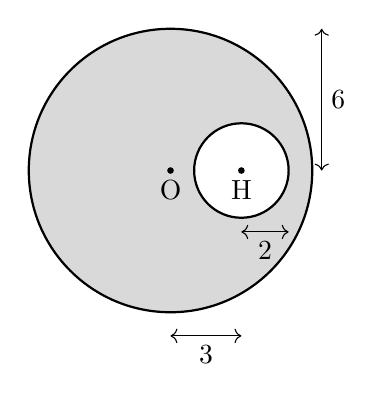
\begin{tikzpicture}[scale=0.6]
% Draw large circle
\draw[thick, fill=gray!30] (0,0) circle (3);
% Draw hole
\draw[thick, fill=white] (1.5,0) circle (1);

% Mark centers
\fill (0,0) circle (2pt) node[below] {O};
\fill (1.5,0) circle (2pt) node[below] {H};

% Add dimensions
\draw[<->] (3.2,0) -- (3.2,3) node[midway, right] {6};
\draw[<->] (1.5,-1.3) -- (2.5,-1.3) node[midway, below] {2};
\draw[<->] (0,-3.5) -- (1.5,-3.5) node[midway, below] {3};
\end{tikzpicture}
\end{document}
